\documentclass{beamer}
\usetheme{Madrid}
\usecolortheme{default}

% Define OSU orange color
\definecolor{osaorange}{RGB}{220,115,38}

% Set colors
\setbeamercolor{structure}{fg=osaorange}
\setbeamercolor{title}{fg=white,bg=osaorange}
\setbeamercolor{frametitle}{fg=white,bg=osaorange}

% Remove navigation symbols
\setbeamertemplate{navigation symbols}{}

\usepackage{graphicx}
\usepackage{amsmath}
\usepackage{booktabs}
\usepackage{hyperref}
\usepackage{tikz}
\usetikzlibrary{shapes,arrows}

\title{H524 Introduction to Biostatistics}
\subtitle{Week 8: Contingency Tables and Chi-Square Tests}
\author{Dr. John Molitor}
\institute{}
\date{Fall 2025}

\begin{document}

\frame{\titlepage}

\begin{frame}
\frametitle{Outline}
\tableofcontents
\end{frame}

\section{Review: Where We've Been}

\begin{frame}
\frametitle{Quick Review: Weeks 6-7 Recap}
\textbf{Recent Topics Covered:}
\begin{itemize}
\item \textbf{Week 6:} Hypothesis Testing Framework
  \begin{itemize}
  \item One-sample and two-sample t-tests
  \item Paired tests
  \item Type I and Type II errors, power
  \end{itemize}
\item \textbf{Week 7:} Nonparametric Methods
  \begin{itemize}
  \item Sign test, Wilcoxon signed-rank test
  \item Mann-Whitney U test
  \item When to use nonparametric vs parametric tests
  \end{itemize}
\end{itemize}

\vspace{0.5cm}
\textbf{Common theme:} Comparing means (continuous outcomes)

\vspace{0.3cm}
\textbf{This week:} Categorical outcomes and associations
\end{frame}

\begin{frame}
\frametitle{From Continuous to Categorical Data}
\textbf{So far in H524:}
\begin{itemize}
\item Continuous outcomes: blood pressure, cholesterol, pain scores
\item Methods: t-tests, confidence intervals, ANOVA
\item Questions: Are means different between groups?
\end{itemize}

\vspace{0.5cm}
\textbf{New challenge: Categorical outcomes}
\begin{itemize}
\item Binary: disease/no disease, treatment success/failure
\item Nominal: blood type (A, B, AB, O), race/ethnicity
\item Ordinal: disease stage (I, II, III, IV), pain level (none, mild, moderate, severe)
\item Count data: number of deaths, adverse events, cases
\end{itemize}

\vspace{0.5cm}
\textbf{Key Questions:}
\begin{itemize}
\item Is there an association between two categorical variables?
\item Do observed frequencies match expected frequencies?
\item Are two categorical variables independent?
\end{itemize}
\end{frame}

\section{The Origins: Fisher's Tea Experiment}

\begin{frame}
\frametitle{The Lady Tasting Tea (1920s)}
\textbf{The Claim:}
\begin{itemize}
\item Dr. Muriel Bristol, a phycologist at Rothamsted Experimental Station (England)
\item Claimed she could taste whether milk was poured before or after tea
\item Most people thought this was impossible
\end{itemize}

\vspace{0.2cm}
\textbf{The Skeptic:}
\begin{itemize}
\item Sir Ronald A. Fisher, famous English statistician, doubted her claim
\item Proposed testing her claim through a controlled experiment
\item Designed an experiment that would become legendary
\end{itemize}

\vspace{0.2cm}
\textbf{A Foundational Moment in Statistics:}
\begin{itemize}
\item Fisher used this as the famous example for his exact test
\item Original exposition of the null hypothesis concept (1935)
\item Established principles for randomized experiments and hypothesis testing
\end{itemize}

\vspace{0.1cm}
\small{\textit{Note: Rothamsted Experimental Station, England, early 1920s}}
\end{frame}

\begin{frame}
\frametitle{Fisher's Experimental Design}
\textbf{The Setup:}
\begin{itemize}
\item Prepare 8 cups of tea
\item 4 cups: milk poured first, then tea (M$\rightarrow$T)
\item 4 cups: tea poured first, then milk (T$\rightarrow$M)
\item Present all 8 cups in random order
\end{itemize}

\vspace{0.5cm}
\textbf{The Task:}
\begin{itemize}
\item Dr. Bristol must identify which 4 cups are milk-first
\item She knows there are exactly 4 of each type
\item No other cues allowed (temperature, color controlled)
\end{itemize}

\vspace{0.5cm}
\textbf{The Question:}
\begin{itemize}
\item If she's just guessing randomly, what's the probability she gets all 4 correct?
\item This is a question about \textbf{counting combinations}
\end{itemize}
\end{frame}

\begin{frame}
\frametitle{Calculating the Probability}
\textbf{Total possible outcomes:}
\begin{itemize}
\item How many ways can you choose 4 cups from 8?
\item $\binom{8}{4} = \frac{8!}{4! \times 4!} = 70$ different combinations
\end{itemize}

\vspace{0.5cm}
\textbf{Favorable outcomes (all correct):}
\begin{itemize}
\item She correctly identifies all 4 milk-first cups
\item Only 1 way to do this: $\binom{4}{4} \times \binom{4}{0} = 1$
\end{itemize}

\vspace{0.5cm}
\textbf{Probability by pure chance:}
$$p = \frac{1}{70} = 0.0143$$

\vspace{0.3cm}
\textbf{The Result:}
\begin{itemize}
\item Dr. Bristol correctly identified all 8 cups!
\item Probability of this happening by chance: $p = 0.0143$ (less than 5\%)
\item Conclusion: Strong evidence she really could taste the difference
\end{itemize}
\end{frame}

\begin{frame}
\frametitle{Who Was Sir Ronald A. Fisher?}
\textbf{Sir Ronald Aylmer Fisher (1890-1962)}

\vspace{0.2cm}
\textbf{Prominent English Statistician and Geneticist}

\vspace{0.3cm}
\textbf{Foundational Contributions to Statistics:}
\begin{itemize}
\item \textbf{Experimental design:} Randomization, blocking, factorial designs
\item \textbf{Analysis of Variance (ANOVA):} Comparing multiple groups
\item \textbf{Maximum likelihood estimation:} Parameter estimation method
\item \textbf{Fisher's exact test:} Born from the tea experiment
\item \textbf{Genetics:} Reconciled Mendelian genetics with Darwinian evolution
\end{itemize}

\vspace{0.3cm}
\textbf{Career:}
\begin{itemize}
\item Worked at Rothamsted Experimental Station (1919-1933)
\item Later: Professor at University College London and Cambridge
\item One of the most influential scientists of the 20th century
\end{itemize}

\vspace{0.2cm}
\small{\textit{Reference: Fisher, R.A. (1935). The Design of Experiments. Oliver \& Boyd.}}
\end{frame}

\section{Fisher's Exact Test}

\begin{frame}
\frametitle{Fisher's Exact Test: Hypotheses}
\textbf{For a $2 \times 2$ contingency table:}

\vspace{0.3cm}
\begin{center}
\begin{tabular}{l|cc}
& \textbf{Col 1} & \textbf{Col 2} \\
\hline
\textbf{Row 1} & $a$ & $b$ \\
\textbf{Row 2} & $c$ & $d$ \\
\end{tabular}
\end{center}

\vspace{0.5cm}
\textbf{Hypotheses:}
\begin{itemize}
\item $H_0$: The two variables are independent (no association)
\item $H_A$: The two variables are associated (dependent)
\end{itemize}

\vspace{0.5cm}
\textbf{What the p-value tells us:}
\begin{itemize}
\item Probability of seeing a table this extreme (or more) if $H_0$ is true
\item Small p-value $\Rightarrow$ reject $H_0$ $\Rightarrow$ evidence of association
\item Large p-value $\Rightarrow$ fail to reject $H_0$ $\Rightarrow$ no evidence of association
\end{itemize}
\end{frame}

\begin{frame}
\frametitle{Fisher's Exact Test: The Math}
\textbf{For a $2 \times 2$ table:}
\begin{center}
\begin{tabular}{l|cc|c}
& Col 1 & Col 2 & Total \\
\hline
Row 1 & $a$ & $b$ & $a+b$ \\
Row 2 & $c$ & $d$ & $c+d$ \\
\hline
Total & $a+c$ & $b+d$ & $n$ \\
\end{tabular}
\end{center}

\vspace{0.2cm}
\textbf{Exact probability (hypergeometric distribution):}
$$P = \frac{\binom{a+b}{a} \binom{c+d}{c}}{\binom{n}{a+c}}$$

\vspace{0.2cm}
\textbf{The idea:}
\begin{itemize}
\item Calculate probability of observed table (given fixed margins)
\item Calculate probabilities of all more extreme tables
\item Sum these probabilities = exact p-value
\item No approximation needed!
\end{itemize}

\vspace{0.1cm}
\textbf{Note:} Hand calculation tedious; R does it for us
\end{frame}

\begin{frame}[fragile]
\frametitle{Fisher's Exact Test: Example with Tea Data}
\textbf{Representing Dr. Bristol's results as a $2 \times 2$ table:}

\vspace{0.2cm}
\begin{center}
\begin{tabular}{l|cc|c}
& \textbf{Actually M$\rightarrow$T} & \textbf{Actually T$\rightarrow$M} & \textbf{Total} \\
\hline
\textbf{Identified M$\rightarrow$T} & 4 & 0 & 4 \\
\textbf{Identified T$\rightarrow$M} & 0 & 4 & 4 \\
\hline
\textbf{Total} & 4 & 4 & 8 \\
\end{tabular}
\end{center}

\vspace{0.3cm}
\textbf{R code:}
\begin{verbatim}
tea <- matrix(c(4, 0, 0, 4), nrow=2)
fisher.test(tea)
\end{verbatim}

\vspace{0.2cm}
\textbf{Result:} $p = 0.0143$

\vspace{0.2cm}
\textbf{Conclusion:} Strong evidence she could really taste the difference!
\end{frame}

\begin{frame}[fragile]
\frametitle{Fisher's Exact Test: Modern Medical Example}
\textbf{Scenario:} Rare disease study with small sample

\vspace{0.2cm}
\begin{center}
\begin{tabular}{l|cc|c}
& \textbf{Disease} & \textbf{No Disease} & \textbf{Total} \\
\hline
\textbf{Exposed} & 8 & 2 & 10 \\
\textbf{Not Exposed} & 3 & 7 & 10 \\
\hline
\textbf{Total} & 11 & 9 & 20 \\
\end{tabular}
\end{center}

\vspace{0.3cm}
\textbf{R code (replace numbers with your data):}
\begin{verbatim}
data <- matrix(c(8, 2, 3, 7), nrow=2)
fisher.test(data)
\end{verbatim}

\vspace{0.2cm}
\textbf{Result:} P-value = 0.035 (two-sided)

\vspace{0.2cm}
\textbf{Conclusion:} Significant association between exposure and disease

\vspace{0.2cm}
\textbf{When to use:} Small samples (especially when any cell count $<$ 5)
\end{frame}

\begin{frame}
\frametitle{Scaling Up: The Challenge of Large Samples}
\textbf{Fisher's exact test works beautifully for small samples...}

\vspace{0.3cm}
\textbf{But what about large datasets?}
\begin{itemize}
\item Tea experiment: 8 cups → 70 combinations (countable)
\item Medical study: 100 patients → thousands of combinations
\item Large survey: 1000 participants → billions of combinations!
\end{itemize}

\vspace{0.3cm}
\textbf{The Problem:}
\begin{itemize}
\item Counting all combinations becomes computationally expensive
\item Even modern computers struggle with very large samples
\item We need a more efficient approach
\end{itemize}

\vspace{0.3cm}
\textbf{The Solution:}
\begin{itemize}
\item For large samples, we can use a mathematical approximation
\item The hypergeometric distribution approximates the chi-square distribution
\item This gives us the \textbf{chi-square test}
\end{itemize}
\end{frame}

\section{Chi-Square Goodness-of-Fit Test (Ch 15.1)}

\begin{frame}
\frametitle{Introduction to Chi-Square Tests}
\textbf{The chi-square ($\chi^2$) test family:}
\begin{itemize}
\item Tests for categorical data
\item Based on comparing observed vs expected frequencies
\item Large-sample approximation to Fisher's exact test
\end{itemize}

\vspace{0.5cm}
\textbf{Two main types:}
\begin{enumerate}
\item \textbf{Goodness-of-fit test:} Does a single categorical variable follow a specified distribution?
  \begin{itemize}
  \item Example: Are blood types distributed as expected (45\% O, 40\% A, 11\% B, 4\% AB)?
  \end{itemize}
\item \textbf{Test of independence:} Are two categorical variables associated?
  \begin{itemize}
  \item Example: Is smoking status associated with lung cancer?
  \end{itemize}
\end{enumerate}

\vspace{0.5cm}
\textbf{Reading:} Pagano \& Gauvreau Chapters 15-16
\end{frame}

\begin{frame}
\frametitle{Goodness-of-Fit Test: The Basic Idea}
\textbf{Question:} Do observed data match a theoretical distribution?

\vspace{0.3cm}
\textbf{Setup:}
\begin{itemize}\setlength\itemsep{-0.2em}
\item One categorical variable with $k$ categories
\item Null hypothesis specifies expected proportions: $p_1, p_2, \ldots, p_k$
\item Observed counts: $O_1, O_2, \ldots, O_k$ (total $n$)
\item Expected counts: $E_i = np_i$ for each category
\end{itemize}

\vspace{0.3cm}
\textbf{Chi-square test statistic:}
$$\chi^2 = \sum_{i=1}^{k} \frac{(O_i - E_i)^2}{E_i}$$

\vspace{0.2cm}
\textbf{Intuition:}
\begin{itemize}\setlength\itemsep{-0.2em}
\item If observed $\approx$ expected, then $\chi^2$ is small
\item If observed differs from expected, then $\chi^2$ is large
\item Large $\chi^2 \Rightarrow$ reject $H_0$ (poor fit)
\end{itemize}
\end{frame}

\begin{frame}
\frametitle{Chi-Square Distribution}
\textbf{Properties of the $\chi^2$ distribution:}
\begin{itemize}
\item Right-skewed, non-negative values only
\item Determined by degrees of freedom: $df = k - 1$
\item Mean = $df$, Variance = $2 \times df$
\item As $df$ increases, approaches normal distribution
\end{itemize}

\vspace{0.5cm}
\textbf{Assumptions for chi-square tests:}
\begin{enumerate}
\item Random sample
\item Independent observations
\item Expected counts $\geq 5$ in each category
  \begin{itemize}
  \item If violated: combine categories or use Fisher's exact test
  \end{itemize}
\item Sufficiently large sample size
\end{enumerate}

\vspace{0.5cm}
\textbf{R function:} \texttt{pchisq(q, df, lower.tail=FALSE)} for p-values
\end{frame}

\begin{frame}
\frametitle{Example 1: Blood Type Distribution}
\textbf{Scenario:} U.S. population blood type distribution:
\begin{itemize}
\item Type O: 45\%
\item Type A: 40\%
\item Type B: 11\%
\item Type AB: 4\%
\end{itemize}

\vspace{0.3cm}
\textbf{Question:} Does a sample of 200 hospital patients match this distribution?

\vspace{0.3cm}
\textbf{Observed counts:}
\begin{center}
\begin{tabular}{lcccc}
\toprule
Blood Type & O & A & B & AB \\
\midrule
Observed & 85 & 78 & 28 & 9 \\
\bottomrule
\end{tabular}
\end{center}

\vspace{0.3cm}
\textbf{Hypotheses:}
\begin{itemize}
\item $H_0$: Hospital patients have same blood type distribution as general population
\item $H_A$: Distribution differs from general population
\end{itemize}
\end{frame}

\begin{frame}
\frametitle{Example 1: Calculations}
\textbf{Step 1: Calculate expected counts}

Expected: $E_i = n \times p_i$ where $n = 200$

\begin{center}
\begin{tabular}{lcccc}
\toprule
Blood Type & O & A & B & AB \\
\midrule
Observed ($O_i$) & 85 & 78 & 28 & 9 \\
Expected ($E_i$) & 90 & 80 & 22 & 8 \\
\bottomrule
\end{tabular}
\end{center}

\vspace{0.5cm}
\textbf{Step 2: Calculate chi-square statistic}

$$\chi^2 = \frac{(85-90)^2}{90} + \frac{(78-80)^2}{80} + \frac{(28-22)^2}{22} + \frac{(9-8)^2}{8}$$

$$= \frac{25}{90} + \frac{4}{80} + \frac{36}{22} + \frac{1}{8}$$

$$= 0.278 + 0.050 + 1.636 + 0.125 = 2.089$$
\end{frame}

\begin{frame}[fragile]
\frametitle{Example 1: Conclusion}
\textbf{Step 3: Find p-value}

\begin{itemize}
\item Degrees of freedom: $df = k - 1 = 4 - 1 = 3$
\item Test statistic: $\chi^2 = 2.089$
\item P-value: $P(\chi^2_3 > 2.089) = 0.554$
\end{itemize}

\vspace{0.5cm}
\textbf{R code:}
\begin{verbatim}
pchisq(2.089, df=3, lower.tail=FALSE)
# Returns: 0.554
\end{verbatim}

\vspace{0.5cm}
\textbf{Conclusion:}
\begin{itemize}
\item P-value = 0.554 $>$ 0.05
\item Fail to reject $H_0$
\item No evidence that hospital blood type distribution differs from general population
\end{itemize}
\end{frame}

\section{Contingency Tables (Ch 15.2-15.3)}

\begin{frame}
\frametitle{Contingency Tables: Introduction}
\textbf{Contingency table} (cross-tabulation): Displays frequency distribution of two categorical variables

\vspace{0.5cm}
\textbf{General $r \times c$ table:}
\begin{itemize}
\item $r$ rows (levels of variable 1)
\item $c$ columns (levels of variable 2)
\item Cell counts: $O_{ij}$ = observed count in row $i$, column $j$
\item Row totals, column totals, grand total $n$
\end{itemize}

\vspace{0.5cm}
\textbf{Key Question:} Are the two variables independent?

\vspace{0.3cm}
\textbf{Hypotheses:}
\begin{itemize}
\item $H_0$: Row and column variables are independent (no association)
\item $H_A$: Row and column variables are associated (dependent)
\end{itemize}
\end{frame}

\begin{frame}
\frametitle{$2 \times 2$ Contingency Table}
\textbf{Most common case:} Two binary variables

\vspace{0.3cm}
\begin{center}
\begin{tabular}{l|cc|c}
& \textbf{Disease} & \textbf{No Disease} & \textbf{Total} \\
\hline
\textbf{Exposed} & $a$ & $b$ & $a+b$ \\
\textbf{Not Exposed} & $c$ & $d$ & $c+d$ \\
\hline
\textbf{Total} & $a+c$ & $b+d$ & $n$ \\
\end{tabular}
\end{center}

\vspace{0.5cm}
\textbf{Examples:}
\begin{itemize}
\item Exposure (smoking) vs Disease (lung cancer)
\item Treatment (drug vs placebo) vs Outcome (success vs failure)
\item Risk factor (hypertension) vs Event (stroke vs no stroke)
\end{itemize}

\vspace{0.5cm}
\textbf{Measures we can calculate:}
\begin{itemize}
\item Relative risk
\item Odds ratio
\item Chi-square test for independence
\end{itemize}
\end{frame}

\begin{frame}
\frametitle{Where Do Expected Values Come From?}
\textbf{Goal:} Find expected count in cell $a$ (Exposed \& Disease) if independent.

\vspace{0.15cm}
\textbf{Under independence:} $P(\text{Exposed AND Disease}) = P(\text{Exposed}) \times P(\text{Disease})$

\vspace{0.15cm}
\textbf{From the 2×2 table:}
\begin{itemize}\setlength\itemsep{-0.1em}
\item $P(\text{Exposed}) = \frac{a+b}{n}$ (row total)
\item $P(\text{Disease}) = \frac{a+c}{n}$ (column total)
\end{itemize}

\vspace{0.15cm}
\textbf{Expected count in cell $a$:}
$$E_a = n \times \frac{a+b}{n} \times \frac{a+c}{n} = \frac{(a+b)(a+c)}{n}$$

\vspace{0.15cm}
\textbf{General formula:}
$$E_{ij} = \frac{(\text{Row total}) \times (\text{Column total})}{n}$$

\textbf{Key insight:} Expected values show what we'd see if variables were independent.
\end{frame}

\begin{frame}
\frametitle{Chi-Square Test of Independence: Hypotheses}
\textbf{Testing association between two categorical variables}

\vspace{0.5cm}
\textbf{Hypotheses:}
\begin{itemize}
\item $H_0$: The row and column variables are independent (no association)
\item $H_A$: The row and column variables are associated (dependent)
\end{itemize}

\vspace{0.5cm}
\textbf{What the p-value tells us:}
\begin{itemize}
\item If p-value $< \alpha$ (typically 0.05): Reject $H_0$
  \begin{itemize}
  \item Evidence that variables are associated
  \item Observed counts differ significantly from what we'd expect under independence
  \end{itemize}
\item If p-value $\geq \alpha$: Fail to reject $H_0$
  \begin{itemize}
  \item No evidence of association
  \item Observed counts consistent with independence
  \end{itemize}
\end{itemize}

\vspace{0.3cm}
\textbf{Note:} Chi-square test tells us IF there's an association, not HOW STRONG it is (use effect sizes for that)
\end{frame}

\begin{frame}
\frametitle{Chi-Square Test of Independence: Formula}
\textbf{Test statistic for $r \times c$ table:}

$$\chi^2 = \sum_{i=1}^{r} \sum_{j=1}^{c} \frac{(O_{ij} - E_{ij})^2}{E_{ij}}$$

\vspace{0.2cm}
\textbf{Expected count formula:}
$$E_{ij} = \frac{(\text{Row } i \text{ total}) \times (\text{Column } j \text{ total})}{\text{Grand total}}$$

\vspace{0.3cm}
\textbf{Degrees of freedom:}
$$df = (r - 1) \times (c - 1)$$

\vspace{0.3cm}
\textbf{Interpretation:}
\begin{itemize}\setlength\itemsep{-0.2em}
\item Expected counts assume independence (null hypothesis)
\item Large differences between $O_{ij}$ and $E_{ij} \Rightarrow$ evidence of association
\item Compare $\chi^2$ to chi-square distribution with appropriate $df$
\end{itemize}
\end{frame}

\begin{frame}
\frametitle{Example 3: Smoking and Lung Cancer}
\textbf{Case-control study:} 100 lung cancer patients, 100 controls

\vspace{0.3cm}
\begin{center}
\begin{tabular}{l|cc|c}
& \textbf{Lung Cancer} & \textbf{No Cancer} & \textbf{Total} \\
\hline
\textbf{Smoker} & 85 & 55 & 140 \\
\textbf{Non-smoker} & 15 & 45 & 60 \\
\hline
\textbf{Total} & 100 & 100 & 200 \\
\end{tabular}
\end{center}

\vspace{0.5cm}
\textbf{Question:} Is there an association between smoking and lung cancer?

\vspace{0.3cm}
\textbf{Hypotheses:}
\begin{itemize}
\item $H_0$: Smoking status and lung cancer are independent
\item $H_A$: Smoking status and lung cancer are associated
\end{itemize}
\end{frame}

\begin{frame}
\frametitle{Example 3: Expected Counts}
\textbf{Calculate expected counts under independence:}

$$E_{ij} = \frac{(\text{Row total}) \times (\text{Column total})}{n}$$

\vspace{0.3cm}
\begin{center}
\begin{tabular}{l|cc}
& \textbf{Cancer} & \textbf{No Cancer} \\
\hline
\textbf{Smoker} & $\frac{140 \times 100}{200} = 70$ & $\frac{140 \times 100}{200} = 70$ \\
\textbf{Non-smoker} & $\frac{60 \times 100}{200} = 30$ & $\frac{60 \times 100}{200} = 30$ \\
\end{tabular}
\end{center}

\vspace{0.5cm}
\textbf{Summary table:}
\begin{center}
\begin{tabular}{lcc}
\toprule
Cell & Observed & Expected \\
\midrule
Smoker + Cancer & 85 & 70 \\
Smoker + No Cancer & 55 & 70 \\
Non-smoker + Cancer & 15 & 30 \\
Non-smoker + No Cancer & 45 & 30 \\
\bottomrule
\end{tabular}
\end{center}
\end{frame}

\begin{frame}
\frametitle{Example 3: Chi-Square Calculation}

\textbf{Observed counts with expected in parentheses:}
\begin{center}
\begin{tabular}{l|cc}
& \textbf{Cancer} & \textbf{No Cancer} \\
\hline
\textbf{Smoker} & 85 \textcolor{red}{(70)} & 55 \textcolor{red}{(70)} \\
\textbf{Non-smoker} & 15 \textcolor{red}{(30)} & 45 \textcolor{red}{(30)} \\
\end{tabular}
\end{center}

\vspace{0.3cm}
\textbf{Calculate $\chi^2$:}
\small
$$\chi^2 = \sum \frac{(O-E)^2}{E} = \frac{(85-70)^2}{70} + \frac{(55-70)^2}{70} + \frac{(15-30)^2}{30} + \frac{(45-30)^2}{30}$$

$$= 3.21 + 3.21 + 7.50 + 7.50 = 21.43$$

\normalsize
$df = 1$, p-value $< 0.0001$ $\Rightarrow$ \textbf{Very strong evidence of association}
\end{frame}

\begin{frame}
\frametitle{Example 4: Treatment Efficacy}
\textbf{Clinical trial:} New drug vs placebo for treating infection

\vspace{0.3cm}
\textbf{Observed counts with expected in parentheses:}
\begin{center}
\begin{tabular}{l|cc|c}
& \textbf{Cured} & \textbf{Not Cured} & \textbf{Total} \\
\hline
\textbf{Drug} & 48 \textcolor{red}{(40)} & 12 \textcolor{red}{(20)} & 60 \\
\textbf{Placebo} & 32 \textcolor{red}{(40)} & 28 \textcolor{red}{(20)} & 60 \\
\hline
\textbf{Total} & 80 & 40 & 120 \\
\end{tabular}
\end{center}

\vspace{0.3cm}
\textbf{Calculate $\chi^2$:}
$$\chi^2 = \frac{(48-40)^2}{40} + \frac{(12-20)^2}{20} + \frac{(32-40)^2}{40} + \frac{(28-20)^2}{20} = 9.60$$

\vspace{0.2cm}
$df = 1$, p-value = 0.002 $\Rightarrow$ \textbf{Strong evidence drug is more effective}
\end{frame}

\begin{frame}
\frametitle{Larger Contingency Tables}
\textbf{Example:} $3 \times 3$ table - Disease severity by age group

\vspace{0.3cm}
\begin{center}
\begin{tabular}{l|ccc|c}
& \textbf{Mild} & \textbf{Moderate} & \textbf{Severe} & \textbf{Total} \\
\hline
\textbf{Young ($<40$)} & 45 & 20 & 5 & 70 \\
\textbf{Middle (40-60)} & 30 & 35 & 15 & 80 \\
\textbf{Older ($>60$)} & 15 & 25 & 10 & 50 \\
\hline
\textbf{Total} & 90 & 80 & 30 & 200 \\
\end{tabular}
\end{center}

\vspace{0.5cm}
\textbf{Analysis:}
\begin{itemize}
\item $df = (3-1)(3-1) = 4$
\item Calculate 9 expected counts
\item Sum contributions: $\chi^2 = \sum \frac{(O_{ij}-E_{ij})^2}{E_{ij}}$
\item Compare to $\chi^2_4$ distribution
\end{itemize}

\vspace{0.3cm}
\textbf{Interpretation:} Significant result indicates association between age and disease severity, but doesn't specify pattern
\end{frame}


\begin{frame}
\frametitle{Advanced Topic: McNemar's Test for Paired Data}
\textbf{A specialized test for paired/matched binary data}

\vspace{0.5cm}
\textbf{When is it used?}
\begin{itemize}
\item Same subjects measured twice (before/after studies)
\item Matched pairs (twins, matched case-control designs)
\item Any situation where observations are paired
\end{itemize}

\vspace{0.5cm}
\textbf{Why different from chi-square?}
\begin{itemize}
\item Chi-square assumes independent observations
\item McNemar's accounts for the pairing/matching
\item Uses only discordant pairs (subjects who changed)
\end{itemize}

\vspace{0.5cm}
\textbf{For this course:}
\begin{itemize}
\item More advanced test - covered in detail during lab
\item Worksheet Problem 5 is optional practice
\item Important when you encounter paired data in research
\end{itemize}
\end{frame}

\section{Practical Considerations and R Implementation}

\begin{frame}[fragile]
\frametitle{Chi-Square Tests in R (Part 1 - Goodness-of-Fit)}
\textbf{Goodness-of-fit test:}
\begin{verbatim}
# Observed counts
observed <- c(85, 78, 28, 9)
# Expected proportions
expected_props <- c(0.45, 0.40, 0.11, 0.04)

# Chi-square test
chisq.test(observed, p=expected_props)
\end{verbatim}

\vspace{0.5cm}
\textbf{Output includes:}
\begin{itemize}
\item $\chi^2$ statistic
\item Degrees of freedom
\item P-value
\end{itemize}
\end{frame}

\begin{frame}[fragile]
\frametitle{Chi-Square Tests in R (Part 2 - Test of Independence)}
\textbf{Test of independence:}
\begin{verbatim}
# Create contingency table
data <- matrix(c(85, 55, 15, 45), nrow=2, byrow=TRUE)
rownames(data) <- c("Smoker", "Non-smoker")
colnames(data) <- c("Cancer", "No Cancer")

# Chi-square test
chisq.test(data)

# With continuity correction (for 2x2 tables)
chisq.test(data, correct=TRUE)
\end{verbatim}
\end{frame}

\begin{frame}[fragile]
\frametitle{Fisher's Exact Test in R}
\textbf{Fisher's exact test:}
\begin{verbatim}
# For 2x2 table
data <- matrix(c(8, 2, 3, 7), nrow=2)
fisher.test(data)
\end{verbatim}

\vspace{0.5cm}
\textbf{When to use:}
\begin{itemize}
\item Small sample sizes
\item Expected counts $< 5$
\item Exact p-values needed
\end{itemize}
\end{frame}

% ============================================================================
% WEEK 9 PREVIEW (OPTIONAL)
% ============================================================================

\section{Preview: Week 9 - Effect Sizes (Optional)}

\begin{frame}
\frametitle{Preview of Week 9: Effect Sizes}
\begin{center}
\Large \textcolor{blue}{Optional Preview of Next Week}
\end{center}

\vspace{0.3cm}

\textbf{Coming in Week 9:}
\begin{itemize}\setlength\itemsep{0em}
\item Relative Risk (RR)
\item Odds Ratio (OR)
\item Interpreting effect sizes
\item When to use RR vs OR
\end{itemize}

\vspace{0.3cm}

\textbf{Note:} The following slides are optional. Feel free to read ahead!
\end{frame}

\begin{frame}
\frametitle{Effect Sizes: Relative Risk and Odds Ratio (Week 9 Preview)}
\textbf{These measures quantify the strength of association in 2×2 tables}

\vspace{0.3cm}
\textbf{Relative Risk (RR):}
\begin{itemize}
\item Ratio of disease risk in exposed vs unexposed groups
\item $RR = \frac{a/(a+b)}{c/(c+d)}$ (from 2×2 table)
\item Interpretation: RR = 2.0 means exposed group has twice the risk
\item RR = 1.0 means no association
\end{itemize}

\vspace{0.3cm}
\textbf{Odds Ratio (OR):}
\begin{itemize}
\item Ratio of odds of disease in exposed vs unexposed groups
\item Odds in exposed = $a/b$, odds in unexposed = $c/d$
\item $OR = \frac{a/b}{c/d} = \frac{a}{b} \times \frac{d}{c} = \frac{a \times d}{b \times c}$ (cross-product)
\item Interpretation: OR = 2.0 means exposed group has twice the odds
\item OR = 1.0 means no association
\end{itemize}

\vspace{0.3cm}
\textbf{When to use:} RR for cohort studies, OR for case-control studies
\end{frame}

\begin{frame}[fragile]
\frametitle{Effect Sizes in R (Week 9 Preview)}
\textbf{Odds ratio and confidence interval:}
\begin{verbatim}
# Using fisher.test
result <- fisher.test(data)
result$estimate    # Odds ratio
result$conf.int    # 95% CI

# Manual calculation
OR <- (data[1,1] * data[2,2]) / (data[1,2] * data[2,1])
\end{verbatim}

\vspace{0.5cm}
\textbf{Relative risk (manual):}
\begin{verbatim}
RR <- (data[1,1]/sum(data[1,])) /
      (data[2,1]/sum(data[2,]))
\end{verbatim}
\end{frame}

\begin{frame}[fragile]
\frametitle{Visualizing Contingency Tables (Part 1 - Mosaic Plot)}

\begin{columns}[T]
\begin{column}{0.48\textwidth}
\textbf{R code:}
\small
\begin{verbatim}
# Create data
data <- matrix(c(85, 55, 15, 45),
               nrow=2)
rownames(data) <- c("Smoker",
                    "Non-smoker")
colnames(data) <- c("Cancer",
                    "No Cancer")

# Mosaic plot
mosaicplot(data,
  main="Smoking and Cancer",
  color=c("darkred",
          "lightblue"),
  xlab="Smoking Status",
  ylab="Cancer Status")
\end{verbatim}
\end{column}

\begin{column}{0.48\textwidth}
\textbf{Output:}
\vspace{0.2cm}
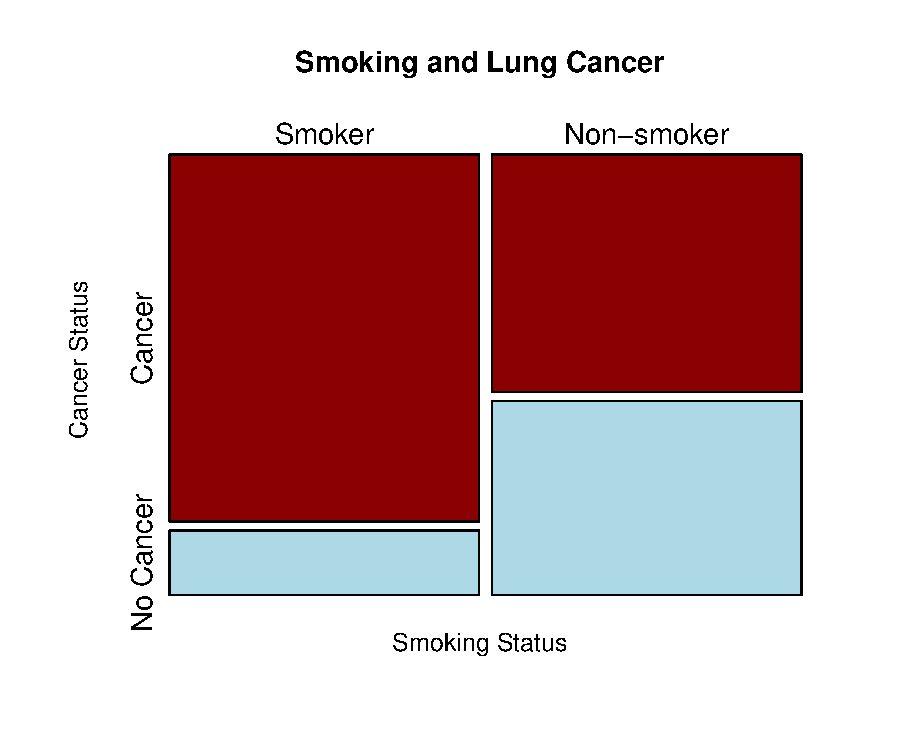
\includegraphics[width=\textwidth]{figures/mosaic_plot.pdf}

\vspace{0.2cm}
\small
Area proportional to cell counts. Shows association visually.
\end{column}
\end{columns}
\end{frame}

\begin{frame}[fragile]
\frametitle{Visualizing Contingency Tables (Part 2 - Counts)}

\begin{columns}[T]
\begin{column}{0.48\textwidth}
\textbf{R code:}
\small
\begin{verbatim}
barplot(data, beside=TRUE,
        legend=TRUE,
        col=c("darkred",
              "darkgreen"),
        main="Smoking and Cancer",
        xlab="Cancer Status",
        ylab="Count")
\end{verbatim}

\vspace{0.3cm}
Shows absolute counts side-by-side for comparison.
\end{column}

\begin{column}{0.48\textwidth}
\textbf{Output:}
\vspace{0.2cm}
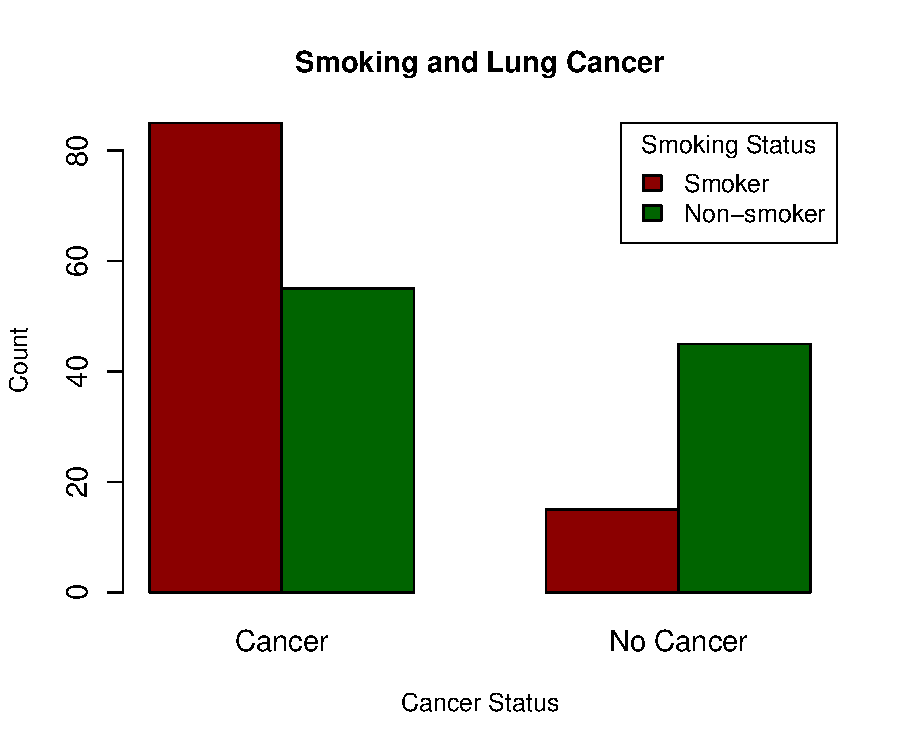
\includegraphics[width=\textwidth]{figures/barplot_counts.pdf}
\end{column}
\end{columns}
\end{frame}

\begin{frame}[fragile]
\frametitle{Visualizing Contingency Tables (Part 3 - Proportions)}

\begin{columns}[T]
\begin{column}{0.48\textwidth}
\textbf{R code:}
\small
\begin{verbatim}
# Row proportions
prop_data <- prop.table(data,
                        margin=1)

barplot(prop_data,
        beside=TRUE,
        legend=TRUE,
        col=c("darkred",
              "darkgreen"),
        main="Cancer Rates",
        ylab="Proportion")
\end{verbatim}

\vspace{0.3cm}
Shows cancer rates within each smoking group.
\end{column}

\begin{column}{0.48\textwidth}
\textbf{Output:}
\vspace{0.2cm}
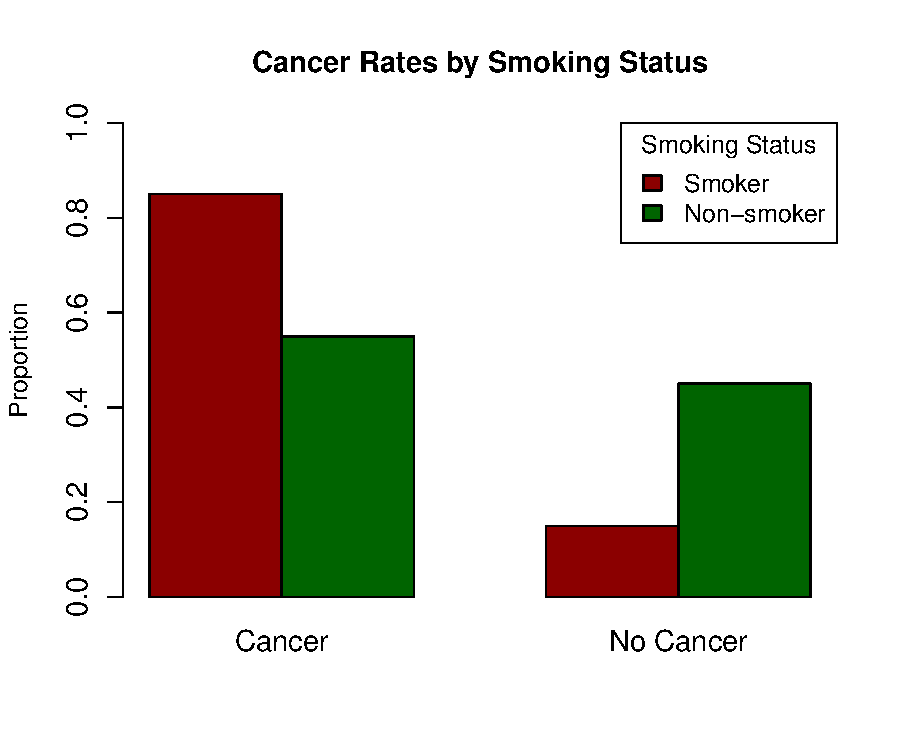
\includegraphics[width=\textwidth]{figures/barplot_proportions.pdf}

\vspace{0.2cm}
\small
Easier to see association: smokers have higher cancer proportion.
\end{column}
\end{columns}
\end{frame}

\begin{frame}
\frametitle{Common Mistakes and Pitfalls}
\textbf{1. Using chi-square with small expected counts}
\begin{itemize}\setlength\itemsep{-0.2em}
\item Check all expected counts $\geq 5$
\item If violated: use Fisher's exact test or combine categories
\end{itemize}

\vspace{0.2cm}
\textbf{2. Confusing association with causation}
\begin{itemize}\setlength\itemsep{-0.2em}
\item Chi-square shows association, not causation
\item May be confounding variables
\end{itemize}

\vspace{0.2cm}
\textbf{3. Using chi-square for paired/matched data}
\begin{itemize}\setlength\itemsep{-0.2em}
\item Independence assumption violated
\item Use McNemar's test instead
\end{itemize}

\vspace{0.2cm}
\textbf{4. Ignoring effect size}
\begin{itemize}\setlength\itemsep{-0.2em}
\item Significant p-value doesn't mean strong association
\item Always examine the actual counts and proportions
\item Effect sizes (OR, RR) covered next week
\end{itemize}

\vspace{0.2cm}
\textbf{5. Multiple testing without adjustment}
\begin{itemize}\setlength\itemsep{-0.2em}
\item Testing many pairs in large tables inflates Type I error
\item Consider Bonferroni or other corrections
\end{itemize}
\end{frame}

\begin{frame}
\frametitle{Choosing the Right Test}

\textbf{One categorical variable vs expected distribution}
\begin{itemize}
\item Chi-square goodness-of-fit
\end{itemize}

\textbf{Two independent categorical variables (large sample)}
\begin{itemize}
\item Chi-square test of independence
\end{itemize}

\textbf{Two independent categorical variables (small sample)}
\begin{itemize}
\item Fisher's exact test
\end{itemize}

\textbf{Paired/matched binary data}
\begin{itemize}
\item McNemar's test
\end{itemize}

\textbf{Ordinal variables with natural ordering}
\begin{itemize}
\item Consider Cochran-Armitage trend test
\end{itemize}

\textbf{Multiple categorical variables}
\begin{itemize}
\item Log-linear models (beyond this course)
\end{itemize}
\end{frame}

\end{document}
